\documentclass{article}
\usepackage[utf8]{inputenc}
\usepackage[margin=0.75in]{geometry}
\usepackage{enumerate}
\usepackage{amsmath}
\usepackage{amsfonts} 
\usepackage{amssymb}
\usepackage{amsthm}
\usepackage{mathtools}
\usepackage{float}
\usepackage{array}
\usepackage{makecell}
\usepackage{commath}
\usepackage{verbatim}

\DeclarePairedDelimiter{\ceil}{\lceil}{\rceil}

\renewcommand\theadalign{bc}
\renewcommand\theadfont{\bfseries}
\renewcommand\theadgape{\Gape[4pt]}
\renewcommand\cellgape{\Gape[4pt]}

\newcommand{\N}{\mathbb{N}}
\newcommand{\Z}{\mathbb{Z}}
\newcommand{\Q}{\mathbb{Q}}
\newcommand{\C}{\mathbb{C}}
\newcommand{\R}{\mathbb{R}}
\newcommand{\F}{\mathbb{F}}
\newtheorem{theorem}{Theorem}
\newtheorem{corollary}{Corollary}[theorem]
\newtheorem{definition}{Definition}[theorem]
\newtheorem{lemma}[theorem]{Lemma}
\newtheorem*{remark}{Remark}
\newcommand{\cdotscalar}{\;\widetilde{\cdot}\;}
\newcommand{\vectorplus}{\;\widetilde{+}\;}
\newcommand{\Span}{\text{Span}}
\newcommand{\Null}{\text{Null}}
\newcommand{\Range}{\text{Range}}
\newcommand{\D}{\frac{d}{\dif x}}

\renewcommand{\epsilon}{\varepsilon}
\renewcommand{\phi}{\varphi}

\newcommand{\Or}{\mbox{ OR }}
\renewcommand{\And}{\mbox{ AND }}
\newcommand{\Not}{\mbox{NOT }}
\newcommand{\Iff}{\mbox{ IFF }}

\newcommand{\Width}{\textup{width}}
\newcommand{\Mesh}{\textup{mesh}}
\newcommand{\Int}{\textup{Int}}
\newcommand{\Ext}{\textup{Ext}}
\newcommand{\Bd}{\textup{Bd}}


\newcommand\widebar[1]{\mathop{\overline{#1}}}
\newcommand*\closure[1]{\widebar{#1}}

\newcommand\Ball[2]{U(#1; #2)}

\begin{document}

\section*{Question 2: Feature Maps}

\begin{enumerate}[(a)]
    \item This data is not seperable by a linear classifier. We know that a linear classifier separating this data must partition $\R^2$ into half-spaces $H_1$ (positive) and $H_0$ (negative) based on a threshold $t$. 
    
    In this dataset, $p_1 = (-2, -1)$ and $p_2 = (2, 3)$ have label $1$, and so are in $H_1$. We know that half-spaces are convex, and so any convex combination of $p_1$ and $p_2$ must lie in $H_1$. If we take $\lambda = 3/4$, then 

    \[p_2 = p_1 + \lambda(p_2 - p_1) = (-2, -1) + \frac{3}{4}(2 - (-2), 3 - (-1)) = (-2, -1) + \frac{3}{4}(4, 4) = (1, 2)\]

    must lie in $H_1$ since it is convex combination of $p_1$ and $p_2$. However, we know that $p_3$ has label $0$, and so must lie in $H_0$. This is a contradiction, and so no linear classifier can separate this data.
    \item We will assume that a threshold $t = 0$ is used. The constraints are as follows:
    
    \begin{align}
        -2w_1 + w_2 &\geq 0\\
        w_1 + 4 w_2 &< 0\\
        2w_1 + 9w_2 &\geq 0
    \end{align}
    \item The feasible area is given by the intersection of the blue, red, and green half-spaces below, which is the shaded region to the left of the red line, above the green line, and below the blue line. The feasible area is shown in Figure \ref{fig:q2c}.
    
    \begin{figure}[H]
        \centering
        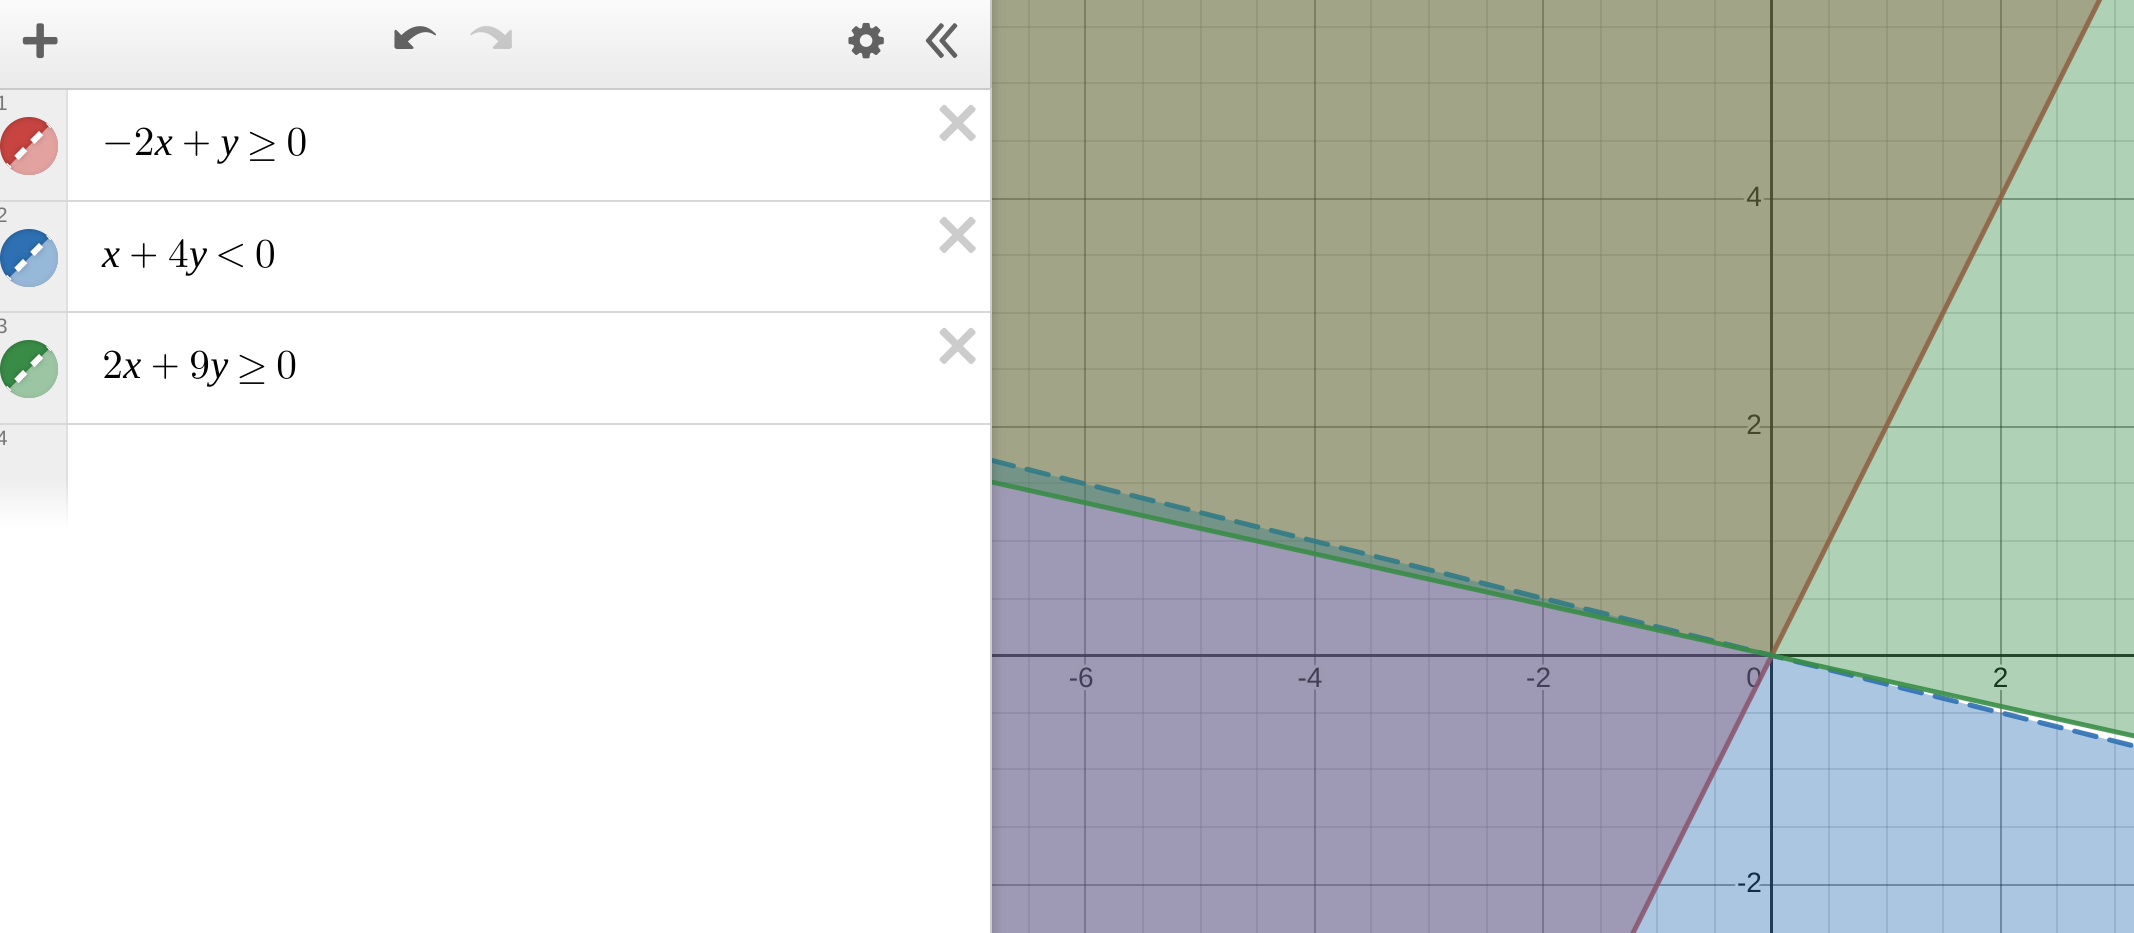
\includegraphics[width=0.9\textwidth]{../figures/q2_c_feasible_area.png}
        \caption{Feasible area for $w_1, w_2$}
        \label{fig:q2c}
    \end{figure}
\end{enumerate}

\newpage
\section*{Question 3: kNN vs Logistic Regression}

\begin{enumerate}[3.1]
    \item \begin{enumerate}[(a)]
        \item The plot of classification vs validation accuracy is given below in Figure \ref{fig:q3a}.
        
        \begin{figure}[H]
            \centering
            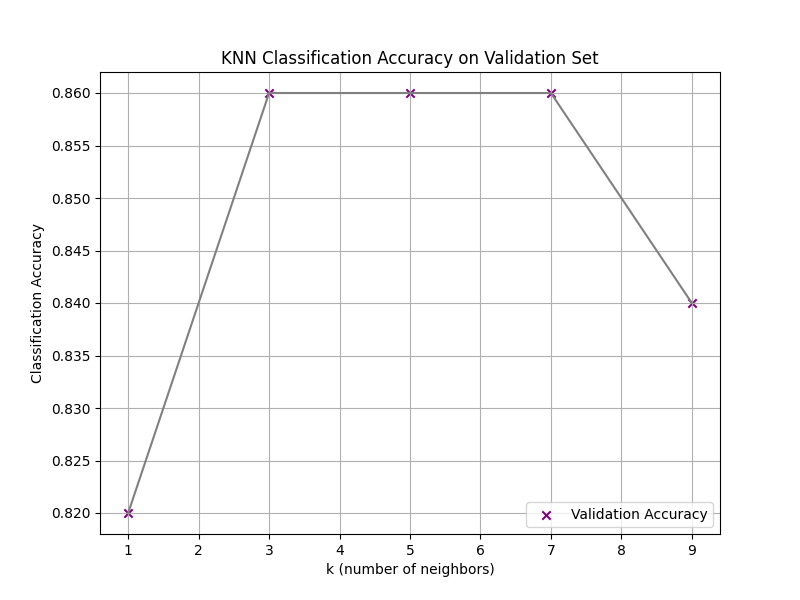
\includegraphics[width=0.7\textwidth]{../figures/knn_classification_accuracy.png}
            \caption{Classification vs Validation Accuracy}
            \label{fig:q3a}
        \end{figure}
    
        \item The value of $k^*$ chosen is $k^* = 3$. This is because $3$ is the smallest value of the hyperparameter $k$ which achieves the maximum accuracy seen across all values of $k$ (0.860). I have chosen this value of $k$ in adherence with the principle of Occam's Razor, which states that the simplest solution is often the best one. In this case, the simplest solution is the least complex model (lowest $k$), as the model complexity increases with $k$. 
        
        Here is a report of the validation and test accuracies for $k^*, k^* + 2, k^* - 2$:
    
        \begin{verbatim}
            Classification accuracies for k_star=3
                Validation accuracy: 0.86
                Test accuracy: 0.92
            Classification accuracies for (k    _star + 2)=5
                Validation accuracy: 0.86
                Test accuracy: 0.94
            Classification accuracies for (k_star - 2)=1
                Validation accuracy: 0.82
                Test accuracy: 0.88
        \end{verbatim}
    
        We see that the maximum validation accuracy is reached when $k^* = 3$, increasing from 0.82 when $k = 1$ and staying at the same value of 0.86 when $k = 5$.
        
        However, the test accuracy increases from $0.88$ to $0.92$ when going from $k^* - 2$ to $k^*$, and continues to increase with $k = k^* + 2 = 5$. This illustrates that the simplest model that performs best on the validation set may not always be the one that performs best on the test set. 
    \end{enumerate}
    
    \item \begin{enumerate}[(a)]
        \item Done!
        \item I've completed the missing parts in \texttt{run\_logistic\_regression}, and run the code on both \texttt{mnist\_train} and \texttt{mnist\_train\_small}. The value returned by \texttt{run\_check\_grad} is small, and is given below:
        
        \begin{verbatim}
            diff = 2.246931370781212e-08
        \end{verbatim}

        I used an initial value of $w = \vec{0}$, and a learning rate of $\eta = 0.2$. I tried values in the range $\{0.1, \dots, 1.0\}$, and I chose this value as it was the largest value of $\eta$ that did not cause the loss to fluctuate in the early training iterations on both the training and validation sets. 

        I used $500$ iterations, as it appears that both the cross entropy and classification accuracies converge on the training and validation sets after $500$ iterations.

        The cross entropy and classification accuracies for the training and validation sets for $\eta = 0.2$ and $500$ iterations are given below:

        \begin{verbatim}
            Classification accuracy on training set: 1.0
            Classification accuracy on validation set: 0.88
            Classification accuracy on test set: 0.92
            Cross entropy on training set: 0.02149375612870086
            Cross entropy on validation set: 0.19186085743772488
            Cross entropy on test set: 0.2142534589131518
        \end{verbatim}

        \item Here are figures showing how cross-entropy changes as training progresses, one for the \texttt{mnist\_train} and one for the \texttt{mnist\_train\_small} datasets.
        
        \begin{figure}[H]
            \centering
            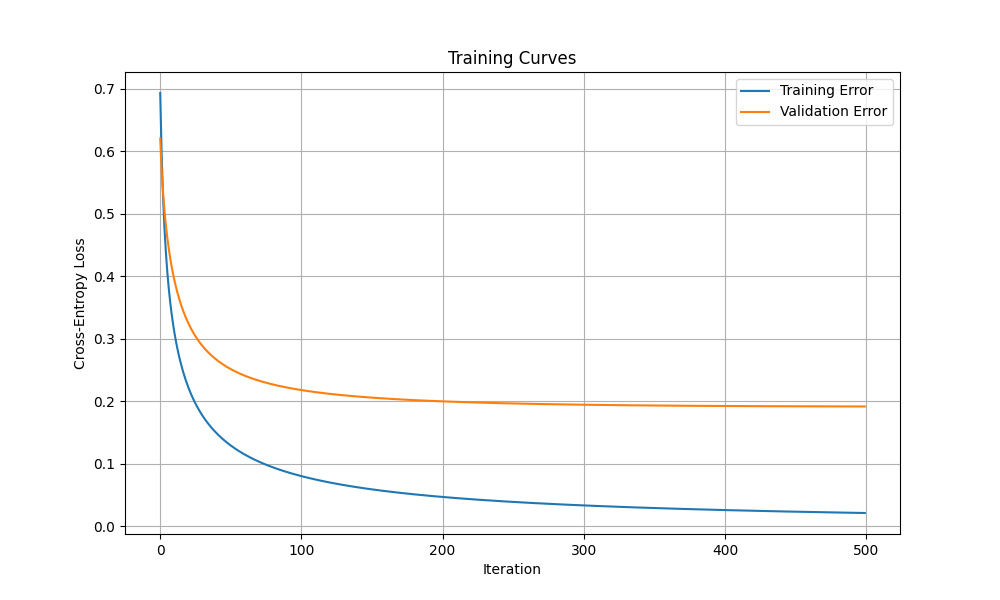
\includegraphics[width=0.7\textwidth]{../figures/mnist_train.png}
            \caption{Cross entropy vs Training Iterations for \texttt{mnist\_train}}
            \label{fig:q3b_mnist_train_cross_entropy}
        \end{figure}

        \begin{figure}[H]
            \centering
            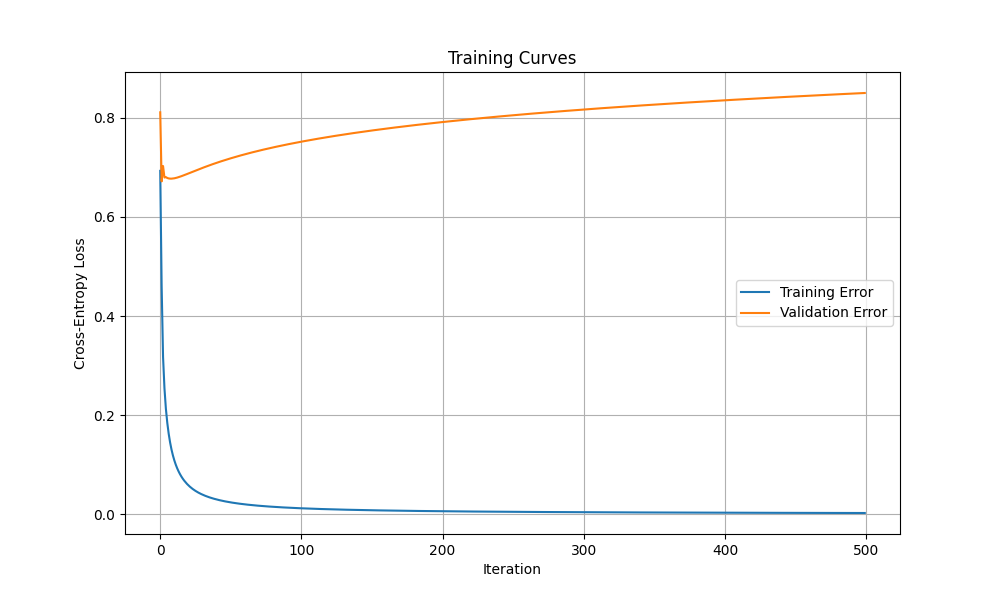
\includegraphics[width=0.7\textwidth]{../figures/mnist_train_small.png}
            \caption{Cross entropy vs Training Iterations for \texttt{mnist\_train\_small}}
            \label{fig:q3b_mnist_train_small_cross_entropy}
        \end{figure}

        We see that the validation error increases as the model trains on \texttt{mnist\_train\_small}, indicating that overfitting is taken place. No such phenomena is observed for \texttt{mnist\_train}, indicating that the model is not overfitting on this dataset.

        From running the code multiple times, we see that the results change slightly. This is due to the random initialization of weights $(w)$ in the function \texttt{run\_logistic\_regression}. One way to choose the best hyperparameter that is the weight initialization is to run the code multiple times, and choose the weight initialization that gives the best validation accuracy.

    \end{enumerate}
\end{enumerate}

\newpage
\section*{Question 4: Locally Weighted Regression}

\begin{enumerate}[(a)]
    \item First, define 
    
    \[J(w) = \frac{1}{2} \sum_{i = 1}^N a^{(i)}(y^{(i)} - w^T x^{(i)})^2 + \frac{\lambda}{2} \norm{w}^2 = \frac{1}{2} \langle y - Xw, A(y - Xw)  \rangle + \frac{\lambda}{2} \langle w , w \rangle \]

    We'll calculate the gradient of $J$ by first finding its Jacobian, and then taking the transpose. We will use the following identities:

    \begin{align*}
        \partial_x \langle x, A \cdot x \rangle &= x^T (A + A^T) = 2x^T A \qquad \text{if $A$ is symmetric} \\
        \partial_x (A - Bx) &= -B \\
    \end{align*}

    We compute the Jacobian as follows:

    \begin{align*}
        \partial J(w) &= \frac{1}{2} \partial \langle y - Xw, A(y - Xw)  \rangle + \frac{\lambda}{2} \partial \langle w , w \rangle \\
        &= (y - Xw)^T \cdot A \cdot (-X) + \lambda w^T \\
        &= (y - Xw)^T (-AX) + \lambda w^T \\
    \end{align*}

    Taking the transpose, we get

    \begin{align*}
        \nabla_w J(w) &= -X^T A^T (y - Xw) + \lambda w \\
    \end{align*}

    Since $J$ is convex, its minimum can be found by setting its gradient to $0$ and solving for $w$. We do this as follows:

    \begin{align*}
        \nabla_w J(w) &= 0 \\
        -X^T A^T (y - Xw) + \lambda w &= 0 \\
        -X^T A^T y + X^T A^T X w + \lambda w &= 0 \\
        (X^T A^T X + \lambda I) w &= X^T A^T y \\
        w &= (X^T A^T X + \lambda I)^{-1} X^T A^T y \\
        &= (X^T A X + \lambda I)^{-1} X^T A y \qquad \text{since $A$ is symmetric}
    \end{align*}

    which shows the desired closed-form solution. 

    \item Done!
    
    \item Here are the training and validation losses as a function of $\tau$:
    
    \begin{figure}[H]
        \centering
        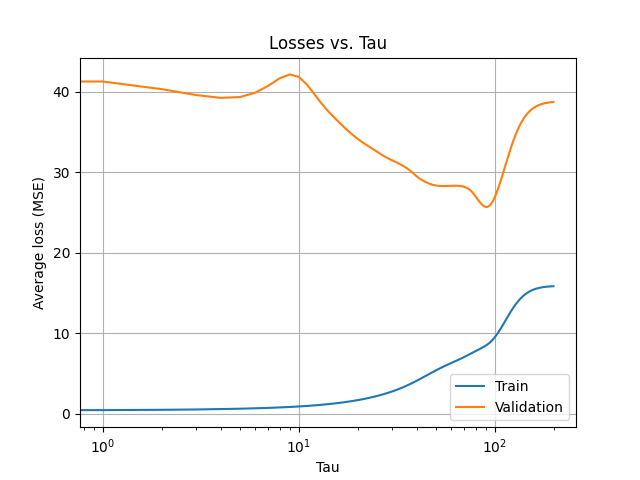
\includegraphics[width=0.7\textwidth]{../figures/q4.png}
        \caption{Training and Validation Losses vs $\tau$}
        \label{fig:q4c_tau_vs_loss}
    \end{figure}

    \item By Lemma 1 below, we see that as $\tau \to 0$, the matrix $A$ contains $1$ in the $i$th diagonal entry if and only if $x^{(i)}$ is the closest point to $x$, and zeroes otherwise. Thus, in this case, our algorithm behaves like a $k$-nearest neighbors model with $k = 1$, since it only trains with respect to the closest point to $x$.
    
    By Lemma 2, we see that as $\tau \to \infty$, the matrix $A$ is given by $I/N$, where $I$ is the identity matrix of size $N \times N$. Thus, in this case, our algorithm behaves exactly like a linear regressor since it weights each point exactly the same and performs linear regression. Indeed, the closed-form solution in part (b) reduces to the closed-form solution for linear regression when $A = I/N$.
    
    \begin{lemma}
        If the distances $\norm{x - x^{(j)}}$ are distinct across all $j$, then \[ \lim_{\tau \to 0} a^{(i)} = \lim_{\tau \to 0}  \frac{\exp\left(-\norm{x - x^{(i)}}^2 /2\tau^2 \right)}{\sum_{j} \exp\left(-\norm{x - x^{(j)}}^2 /2\tau^2\right)} = \begin{cases}
            1 & \text{if $i = \textup{argmin}_j \norm{x - x^{(j)}}^2$} \\
            0 & \text{otherwise}
        \end{cases} \]
    \end{lemma}

    \begin{proof}
        % This can be shown inductively through repeated applications of L'Hopital's rule. We have that

        % \begin{align*}
        %     \lim_{\tau \to 0}  \frac{\exp\left(-\norm{x - x^{(i)}}^2 /2\tau^2 \right)}{\sum_{j} \exp\left(-\norm{x - x^{(j)}}^2 /2\tau^2\right)} &= \lim_{\tau \to 0} \frac{\norm{x - x^{(i)}}^2 \exp\left(-\norm{x - x^{(i)}}^2 /2\tau^2 \right)}{\sum_{j} \norm{x - x^{(j)}}^2 \exp\left(-\norm{x - x^{(j)}}^2 /2\tau^2\right)} \\
        % \end{align*}

        % and by induction, also that 

        % \begin{align*}
        %     \lim_{\tau \to 0}  \frac{\exp\left(-\norm{x - x^{(i)}}^2 /2\tau^2 \right)}{\sum_{j} \exp\left(-\norm{x - x^{(j)}}^2 /2\tau^2\right)} &= \lim_{\tau \to 0} \frac{\norm{x - x^{(i)}}^{2n} \exp\left(-\norm{x - x^{(i)}}^2 /2\tau^2 \right)}{\sum_{j} \norm{x - x^{(j)}}^{2n} \exp\left(-\norm{x - x^{(j)}}^2 /2\tau^2\right)} \\
        % \end{align*}

        % and if $i = \textup{argmin}_j \norm{x - x^{(j)}}^2$, then there exists $n$ such that $\norm{x - x^{(j)}}/\norm{x - x^{(j)}}$ can be made arbitrarily small for all $j \neq i$. Thus, we have in this case that

        % \begin{align*}
        %     \lim_{\tau \to 0}  \frac{\exp\left(-\norm{x - x^{(i)}}^2 /2\tau^2 \right)}{\sum_{j} \exp\left(-\norm{x - x^{(j)}}^2 /2\tau^2\right)} &= \lim_{\tau \to 0} \lim_{n \to \infty}  \frac{\norm{x - x^{(i)}}^{2n} \exp\left(-\norm{x - x^{(i)}}^2 /2\tau^2 \right)}{\sum_{j} \norm{x - x^{(j)}}^{2n} \exp\left(-\norm{x - x^{(j)}}^2 /2\tau^2\right)} \\
        %     &= \lim_{\tau \to 0} \frac{\norm{x - x^{(i)}}^{2n} \exp\left(-\norm{x - x^{(i)}}^2 /2\tau^2 \right)}{\norm{x - x^{(i)}}^{2n} \exp\left(-\norm{x - x^{(i)}}^2 /2\tau^2 \right)}\\
        %     &= 1
        % \end{align*}

        % Similarly, in the case that $i \neq \textup{argmin}_j \norm{x - x^{(j)}}^2$, then 

        % \begin{align*}
        %     \lim_{\tau \to 0}  \frac{\exp\left(-\norm{x - x^{(i)}}^2 /2\tau^2 \right)}{\sum_{j} \exp\left(-\norm{x - x^{(j)}}^2 /2\tau^2\right)} &= \lim_{\tau \to 0} \lim_{n \to \infty}  \frac{\norm{x - x^{(i)}}^{2n} \exp\left(-\norm{x - x^{(i)}}^2 /2\tau^2 \right)}{\sum_{j} \norm{x - x^{(j)}}^{2n} \exp\left(-\norm{x - x^{(j)}}^2 /2\tau^2\right)} \\
        %     &= \lim_{\tau \to 0} \frac{0}{\exp\left(-\norm{x - x^{(k)}}^2 /2\tau^2 \right)} \qquad \text{where $k$ is the minimizer}\\
        %     &= 1
        % \end{align*}

        First, let's divide by $\exp\left(-\norm{x - x^{(i)}}^2 /2\tau^2 \right)$ to get

        \begin{align*}
            \lim_{\tau \to 0}  \frac{\exp\left(-\norm{x - x^{(i)}}^2 /2\tau^2 \right)}{\sum_{j} \exp\left(-\norm{x - x^{(j)}}^2 /2\tau^2\right)} &= \lim_{\tau \to 0} \frac{1}{1 + \sum_{j \neq i} \exp\left(\frac{\norm{x - x^{(i)}} - \norm{x - x^{(j)}}^2}{2\tau^2}\right)} \\
        \end{align*}

        Let's assume that $i = \textup{argmin}_j \norm{x - x^{(j)}}^2$. Then, we have that for $j \neq i$, the argument of the exponential is negative, and goes to $-\infty$ as $\tau \to 0$. Thus, we have that

        \[\lim_{\tau \to 0} a^{(i)} = \frac{1}{1 + 0} = 1 \qquad \text{if } i = \textup{argmin}_j \norm{x - x^{(j)}}^2\]

        Conversely, if $i \neq \textup{argmin}_j \norm{x - x^{(j)}}^2$, then we have that for $j \neq i$, the argument of the exponential is positive, and goes to $\infty$ as $\tau \to 0$. Thus, we have that

        \[\lim_{\tau \to 0} a^{(i)} = \frac{1}{1 + \infty} = 0 \qquad \text{if } i \neq \textup{argmin}_j \norm{x - x^{(j)}}^2\]

        which completes the proof.



    \end{proof}

    \begin{lemma}
        We have that \[\lim_{\tau \to \infty} a^{(i)} = \lim_{\tau \to \infty} \frac{\exp\left(-\norm{x - x^{(i)}}^2 /2\tau^2 \right)}{\sum_{j} \exp\left(-\norm{x - x^{(j)}}^2 /2\tau^2\right)} = \frac{1}{N}\]
        where $N$ is the number of training examples.
    \end{lemma}

    \begin{proof}
        This is simple, and follows from 

        \begin{align*}
            \lim_{\tau \to \infty} a^{(i)} = \frac{\exp(0)}{\sum_{j} \exp(0)} = \frac{1}{N}
        \end{align*}
    \end{proof}

    \item \textbf{Advantage}: The advantage of using locally weighted regression is that it allows one to train a model that is more expressive than a linear model (in the style of KNN) while still performing some non-trival training process. This training process learns from values of \textit{important} training examples that have high values of $a^{(i)}$. This is in the spirit of linear regression, in which our model learns from training examples that are close to the point we are trying to predict.
    
    \textbf{Disadvantage}:  One disadvantage comes from the curse of dimensionality: if the distances of $x$ to $x^{(j)}$, the training examples, are same due to being in a high-dimensional space, then $a^{(i)}$ will roughly be the same, causing the model to behave like a linear regressor. In this case, there is no benefit to the huge computational expense of \textit{recomputing weights} everytime one wants to make a prediction.
\end{enumerate}

\end{document}